%% =============================================================
%%  Les fréquences — de l'octave au comma
%%  Guide de référence, composé en LaTeX, gravure LilyPond
%% =============================================================
%%
%%  Les tableaux (gravures/freq-*.tex), la figure des écarts, la
%%  gravure de la série des harmoniques et les nombres cités dans le
%%  texte (gravures/freq-valeurs.tex) sont produits par
%%  outils/generer_frequences.py, à partir du modèle des fréquences
%%  (outils/frequences.py), qui vérifie chaque identité avant d'écrire.
%%  Voir le colophon en dernière page.
%%
\documentclass[a4paper,11pt]{article}

\usepackage[top=2.2cm,bottom=2.4cm,left=2.2cm,right=2.2cm]{geometry}
\usepackage[T1]{fontenc}
\usepackage[utf8]{inputenc}
\usepackage[french]{babel}
\usepackage{lmodern}
\usepackage{xcolor}
\usepackage{graphicx}
\usepackage{titlesec}
\usepackage{fancyhdr}
\usepackage{mdframed}
\usepackage{array}
\usepackage{enumitem}
\usepackage{booktabs}
\usepackage{amsmath}
\usepackage{tikz}
\usetikzlibrary{decorations.pathreplacing}
\usepackage{hyperref}

\graphicspath{{gravures/}}

% ---- Couleurs, reprises des deux autres guides -----------------------
\definecolor{navy}{RGB}{18,50,105}
\definecolor{lightnavy}{RGB}{235,241,255}
\definecolor{mygray}{RGB}{110,110,110}
\definecolor{accent}{RGB}{150,40,30}

\hypersetup{colorlinks=true, linkcolor=navy, urlcolor=navy,
  pdftitle={Les fréquences — de l'octave au comma},
  pdfauthor={Fabian Bastin}}

% ---- En-tête et pied -----------------------------------------------
\pagestyle{fancy}
\fancyhf{}
\renewcommand{\headrulewidth}{0.4pt}
\renewcommand{\footrulewidth}{0.4pt}
\fancyhead[L]{\small\bfseries\textcolor{navy}{Les fréquences}}
\fancyhead[R]{\small\textcolor{mygray}{\thepage}}
\fancyfoot[C]{\small\textcolor{mygray}{De l'octave au comma}}

% ---- Titres de section ---------------------------------------------
\newcommand{\navysect}[1]{%
  \colorbox{navy}{%
    \parbox[c][17pt]{\dimexpr\linewidth-2\fboxsep\relax}{%
      \color{white}\hspace{6pt}\bfseries\normalsize #1}}%
}
\titleformat{\section}[block]{\normalfont}{}{0pt}{\navysect}
\titlespacing*{\section}{0pt}{16pt}{10pt}
\titleformat{\subsection}
  {\normalfont\normalsize\bfseries\color{navy}}{\thesubsection}{0.6em}{}
\titlespacing*{\subsection}{0pt}{12pt}{5pt}

% ---- Encadrés --------------------------------------------------------
\newmdenv[linecolor=navy, linewidth=0.5pt, backgroundcolor=lightnavy,
  innertopmargin=6pt, innerbottommargin=6pt,
  innerleftmargin=8pt, innerrightmargin=8pt,
  skipabove=8pt, skipbelow=8pt]{remarque}

% Une expérience à faire au synthétiseur : même encadré, filet rouge.
\newmdenv[linecolor=accent, linewidth=0.5pt, backgroundcolor=white,
  innertopmargin=6pt, innerbottommargin=6pt,
  innerleftmargin=8pt, innerrightmargin=8pt,
  skipabove=8pt, skipbelow=8pt]{ecoute}

% ---- Figure gravée -------------------------------------------------
\newcommand{\gravure}[3]{%
  \par\medskip\noindent
  \begin{minipage}{\linewidth}
    \centering
    \includegraphics[width=#2\linewidth]{#1.cropped.pdf}\\[4pt]
    {\small\itshape\color{mygray} #3}
  \end{minipage}\par\medskip
}

% Légende sous un tableau ou une figure TikZ.
\newcommand{\legende}[1]{\\[4pt]{\small\itshape\color{mygray} #1}}

\usepackage[export]{adjustbox}
\setlist{itemsep=2pt, topsep=4pt, parsep=0pt}

% ---- Le synthétiseur -------------------------------------------------
\newcommand{\synthurl}{https://www.slashbin.net/musique/synth.php}
\newcommand{\synth}{\href{\synthurl}{synthétiseur}}
\newcommand{\touche}[1]{\textsf{\small #1}}   % une touche ou un bouton du synthétiseur

% Les nombres cités dans le texte, calculés et vérifiés par le générateur.
%% Produit par outils/generer_frequences.py — ne pas modifier à la main.

\newcommand{\commaPyth}{23{,}46}
\newcommand{\commaPythRapport}{1{,}0136}
\newcommand{\commaSynt}{21{,}51}
\newcommand{\commaHolder}{22{,}64}
\newcommand{\limma}{90{,}22}
\newcommand{\apotome}{113{,}69}
\newcommand{\tonMaj}{203{,}91}
\newcommand{\tonMin}{182{,}40}
\newcommand{\quinteJuste}{701{,}96}
\newcommand{\quarteJuste}{498{,}04}
\newcommand{\tierceJuste}{386{,}31}
\newcommand{\tiercePyth}{407{,}82}
\newcommand{\quinteMeso}{696{,}58}
\newcommand{\loupPyth}{678{,}49}
\newcommand{\loupMeso}{737{,}64}
\newcommand{\demiTon}{1{,}059463}
\newcommand{\ecartQuinte}{1{,}96}
\newcommand{\ecartTierce}{13{,}69}
\newcommand{\ecartTierceMin}{15{,}64}
\newcommand{\puissanceDouze}{129{,}75}
\newcommand{\spiraleFin}{446{,}00}
\newcommand{\spiraleHz}{6{,}00}
\newcommand{\spiraleArrondie}{660, 495, 743, 557, 835, 626, 470, 705, 529, 793, 595, puis 446}
\newcommand{\septiemeHarm}{31{,}2}
\newcommand{\centHz}{0{,}25}
\newcommand{\periodeLa}{2{,}27}
\newcommand{\miSynth}{659{,}25}
\newcommand{\miJuste}{660}
\newcommand{\doDSynth}{554{,}37}
\newcommand{\doDJuste}{550}
\newcommand{\doDPyth}{556{,}88}
\newcommand{\battQuinte}{1{,}5}
\newcommand{\battTierce}{17{,}5}


\begin{document}

% =====================================================================
\begin{titlepage}
\centering
\vspace*{3cm}
{\Huge\bfseries\color{navy} Les fréquences\par}
\vspace{0.6cm}
{\LARGE\color{navy} De l'octave au comma\par}
\vspace{1.4cm}
{\large Ce que mesurent le ton, le demi-ton et le comma\par}
\vspace{2.5cm}
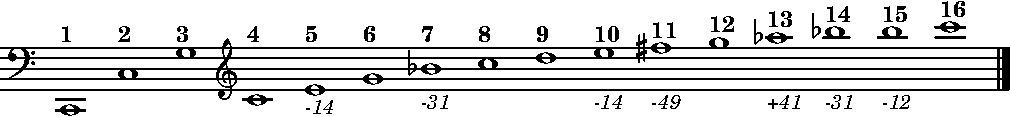
\includegraphics[width=0.85\linewidth]{freq-harmoniques.cropped.pdf}
\vfill
{\small\color{mygray}
Gravure LilyPond, composition \LaTeX.\\
Expériences à faire au synthétiseur de slashbin.net :\\
\url{\synthurl}\par}
\vspace{1cm}
\end{titlepage}

\tableofcontents
\newpage

% =====================================================================
\section{Avant-propos}

Les deux premiers guides,
\href{https://www.slashbin.net/musique/theorie/intervalles.pdf}{\emph{Les
intervalles}} et
\href{https://www.slashbin.net/musique/theorie/gammes.pdf}{\emph{Les gammes}},
comptent en \emph{demi-tons} : une tierce majeure en vaut quatre, une quinte
juste sept. Ils ne disent pas ce qu'est un demi-ton. Celui-ci le dit : une
note est une \textbf{fréquence}, un intervalle un \textbf{rapport} entre deux
fréquences, et l'octave, le ton, le demi-ton et le comma sont des rapports
particuliers, avec une histoire.

On y verra pourquoi l'octave porte deux fois le même nom de note, d'où viennent
le ton et le demi-ton, pourquoi douze quintes ne font pas tout à fait sept
octaves --- c'est le \emph{comma} ---, et comment le piano s'en accommode en
faussant légèrement tous ses intervalles sauf l'octave.

Chaque idée se vérifie à l'oreille avec le \synth{} de slashbin.net, qui joue
une fréquence choisie au hertz près. Les encadrés à filet rouge, comme
celui-ci, proposent une expérience ; la section~\ref{sec:synth} les reprend
toutes, dans l'ordre.

\begin{ecoute}
\textbf{À l'écoute.} Ouvrir \url{\synthurl}, choisir l'onde
\touche{Sinusoïdale}, et appuyer sur la touche \touche{A4} du clavier : c'est le
la du diapason, 440~Hz. Le curseur \touche{Fréquence} se règle aussi au
clavier de l'ordinateur : cliquer dessus, puis les flèches le déplacent d'un
hertz. Une touche du clavier lance le son d'elle-même ; après un réglage au
curseur, il faut appuyer sur \touche{Démarrer}.
\end{ecoute}

\begin{remarque}
\textbf{Conventions.} Les notes sont nommées en français, et les octaves
numérotées à la française : le la du diapason est \emph{la3}, le do du
milieu du piano \emph{do3}. Le synthétiseur, comme la plupart des logiciels,
suit la notation internationale, décalée d'un cran : son \touche{A4} est
notre la3, son \touche{C4} notre do3 (section~\ref{sec:octave}). Les nombres
décimaux s'écrivent avec une virgule ; « Hz » se lit « hertz », vibrations
par seconde.
\end{remarque}

% =====================================================================
\section{Hauteur et fréquence}
\label{sec:frequence}

Un son musical est une vibration de l'air qui se répète. Le nombre de
répétitions par seconde est sa \textbf{fréquence}, mesurée en hertz ; plus
elle est élevée, plus le son est \emph{aigu}. L'oreille humaine entend à peu
près de 20~Hz à 20\,000~Hz ; un piano va du la le plus grave, 27,5~Hz, au do
le plus aigu, environ 4186~Hz.

\textbf{Le diapason.} Pour jouer ensemble, les musiciens s'accordent sur une
fréquence de référence. C'est aujourd'hui le la3 à \textbf{440~Hz}, fixé par
une conférence internationale à Londres en 1939 puis par la norme ISO~16. Il
n'en a pas toujours été ainsi : le « diapason normal » français de 1859
plaçait le la à 435~Hz, la musique baroque se joue souvent à 415~Hz, et bien
des orchestres s'accordent aujourd'hui à 442 ou 443~Hz. Changer de diapason
transpose tout, mais ne change aucun intervalle : ce qui compte, ce sont les
\emph{rapports} entre les notes.

Le mot désigne aussi l'instrument qui donne cette note : une fourche d'acier,
inventée en 1711 par le trompettiste anglais John Shore. Frappées, ses deux
branches vibrent en s'écartant et se rapprochant à une fréquence fixe, et
produisent un son presque pur, sans harmoniques --- celui de l'onde
\touche{Sinusoïdale} du synthétiseur.

% Diapason qui vibre, et l'onde qu'il produit. Dessin TikZ fait à la main :
% rien n'y dépend du modèle, sauf la durée de la période (\periodeLa).
% Un flottant plutôt qu'un bloc centré : trop haut pour la fin de la page 2,
% le bloc passait à la page suivante en laissant un tiers de page vide.
\begin{figure}[tb]
\centering
\begin{tikzpicture}[font=\small]
  % Les branches au repos (plein) et à l'écart maximal (tirets).
  \fill[gray!30, draw=gray!60!black, line width=0.6pt]
    (-0.55,4.2) -- (-0.55,1.6) arc[start angle=180, end angle=360, radius=0.55]
    -- (0.55,4.2) -- (0.33,4.2) -- (0.33,1.6)
    arc[start angle=0, end angle=-180, radius=0.33] -- (-0.33,4.2) -- cycle;
  \draw[gray!60!black, dashed, line width=0.4pt]
    (-0.55,2.2) .. controls (-0.56,3.2) .. (-0.75,4.2) -- (-0.53,4.2)
    .. controls (-0.34,3.2) .. (-0.33,2.2);
  \draw[gray!60!black, dashed, line width=0.4pt]
    (0.55,2.2) .. controls (0.56,3.2) .. (0.75,4.2) -- (0.53,4.2)
    .. controls (0.34,3.2) .. (0.33,2.2);
  % Le manche et sa boule.
  \fill[gray!30, draw=gray!60!black, line width=0.6pt] (-0.11,-0.15) rectangle (0.11,1.06);
  \fill[gray!30, draw=gray!60!black, line width=0.6pt] (0,-0.3) circle (0.2);
  % Le mouvement des branches.
  \draw[<->, accent, thick] (-1.15,3.9) -- (-0.85,3.9);
  \draw[<->, accent, thick] (0.85,3.9) -- (1.15,3.9);
  % Les ondes sonores qui s'éloignent.
  \foreach \r in {1.0,1.45,1.9}
    \draw[navy, thick] (0.6,3.1) ++(-32:\r) arc[start angle=-32, end angle=32, radius=\r];
  \node[below] at (0,-0.55) {\textbf{la3 --- 440~Hz}};
  % L'onde : deux périodes et demie, dont une marquée.
  \begin{scope}[xshift=3.6cm, yshift=2.2cm]
    \draw[->, gray] (0,0) -- (7.3,0) node[right] {temps};
    \draw[->, gray] (0,-1.2) -- (0,1.35) node[above] {pression};
    \draw[navy, thick, domain=0:6.9, samples=200, smooth]
      plot (\x, {sin(\x/2.6*360)});
    % La période, cotée d'une crête à la suivante. La deuxième plutôt que la
    % première : la cote y buterait sur l'étiquette de l'axe.
    \draw[dotted, accent] (3.25,1.05) -- (3.25,1.65);
    \draw[dotted, accent] (5.85,1.05) -- (5.85,1.65);
    \draw[<->, accent, thick] (3.25,1.55) -- (5.85,1.55)
      node[midway, above, font=\footnotesize]
        {une période : $1/440$ de seconde $\approx$ \periodeLa~ms};
  \end{scope}
\end{tikzpicture}\\[4pt]
{\small\itshape\color{mygray} Le diapason. Ses deux branches vibrent
ensemble, l'une contre l'autre, et poussent l'air 440 fois par seconde : la
pression oscille selon une sinusoïde, que l'oreille entend comme le la3.}
\end{figure}

\textbf{L'oreille entend des rapports.} De la2 (220~Hz) à la3 (440~Hz), la
fréquence gagne 220~Hz ; de la3 à la4 (880~Hz), elle en gagne 440. Pourtant
l'oreille entend deux fois le même intervalle, une octave : dans les deux cas,
la fréquence est \emph{doublée}. Un intervalle ne se mesure donc pas par une
différence de fréquences, mais par leur \textbf{rapport} --- la note aiguë
divisée par la grave. Toute la suite découle de cette remarque.

% =====================================================================
\section{L'octave}
\label{sec:octave}

L'\textbf{octave} est le rapport \textbf{2/1} : la note aiguë vibre exactement
deux fois plus vite que la grave. C'est l'intervalle le plus consonant après
l'unisson, au point que deux notes à l'octave portent le même nom. On en verra
la raison avec les harmoniques (section~\ref{sec:harmoniques}) : toutes les
composantes du son aigu se retrouvent dans le son grave.

Monter de $n$ octaves multiplie la fréquence par $2^n$ ; en descendre la divise
par $2^n$. Les do et les la du tableau suivent cette règle d'une ligne à
l'autre.

\begin{center}
%% Produit par outils/generer_frequences.py — ne pas modifier à la main.

\begin{tabular}{@{}c l l r l l r@{}}
\toprule
\textbf{Octave} & \multicolumn{2}{l}{\textbf{Do}} & \textbf{Hz} & \multicolumn{2}{l}{\textbf{La}} & \textbf{Hz} \\
 & \textit{français} & \textit{intern.} & & \textit{français} & \textit{intern.} & \\
\midrule
0 & do0 & C1 & 32{,}70 & la0 & A1 & 55{,}00 \\
1 & do1 & C2 & 65{,}41 & la1 & A2 & 110{,}00 \\
2 & do2 & C3 & 130{,}81 & la2 & A3 & 220{,}00 \\
3 & do3 & C4 & 261{,}63 & la3 & A4 & 440{,}00 \\
4 & do4 & C5 & 523{,}25 & la4 & A5 & 880{,}00 \\
5 & do5 & C6 & 1046{,}50 & la5 & A6 & 1760{,}00 \\
\bottomrule
\end{tabular}

\legende{Les do et les la de six octaves. Le numéro d'octave change au do : le
la3 est au-dessus du do3.}
\end{center}

\begin{remarque}
\textbf{Deux numérotations.} La tradition française numérote les octaves un
cran plus bas que la notation internationale, dite « scientifique ». Le même
son s'écrit donc la3 ou A4, do3 ou C4 ; le la le plus grave du piano, 27,5~Hz,
est le la$-1$ des solfèges français et le A0 international. Le synthétiseur, les logiciels de musique
et la norme MIDI emploient la seconde ; les solfèges français, la première.
Il suffit d'ajouter un au numéro français pour passer à l'international.
\end{remarque}

% =====================================================================
\section{La série des harmoniques}
\label{sec:harmoniques}

Une corde de piano, une colonne d'air dans une flûte, ne vibrent pas à une
seule fréquence. Elles vibrent à la fois à la \emph{fréquence fondamentale}
$f$, qui donne le nom de la note, et à ses multiples entiers $2f$, $3f$, $4f$,
\ldots, de plus en plus faiblement : ce sont les \textbf{harmoniques}. Leur
dosage fait le \emph{timbre} --- ce qui distingue un la de violon d'un la de
clarinette.

\gravure{freq-harmoniques}{0.95}{Les seize premières harmoniques de do1
(65,41~Hz). Sous la note, l'écart en cents à la note tempérée la plus proche,
quand il atteint dix cents : la 7\textsuperscript{e} harmonique est nettement
plus basse que le si bémol du piano.}

Lues dans l'ordre, les harmoniques dessinent les intervalles. Entre les
harmoniques 1 et 2 : une octave, 2/1. Entre 2 et 3 : une quinte, 3/2. Entre 3
et 4 : une quarte, 4/3. Puis la tierce majeure 5/4, la tierce mineure 6/5, et
au-delà des intervalles de plus en plus petits, jusqu'au ton (9/8, 10/9) et
au demi-ton (16/15).

\begin{center}
%% Produit par outils/generer_frequences.py — ne pas modifier à la main.

\begin{tabular}{@{}r r l r c r@{}}
\toprule
\textbf{Rang} & \textbf{Hz} & \textbf{Note tempérée} & \textbf{Écart} & \multicolumn{2}{c}{\textbf{Depuis la précédente}} \\
 & & \textit{la plus proche} & \textit{(cents)} & \textit{rapport} & \textit{cents} \\
\midrule
1 & 65{,}41 & do1 & 0{,}0 &  &  \\
2 & 130{,}81 & do2 & 0{,}0 & 2 & 1200{,}0 \\
3 & 196{,}22 & sol2 & +2{,}0 & 3/2 & 702{,}0 \\
4 & 261{,}63 & do3 & 0{,}0 & 4/3 & 498{,}0 \\
5 & 327{,}03 & mi3 & $-$13{,}7 & 5/4 & 386{,}3 \\
6 & 392{,}44 & sol3 & +2{,}0 & 6/5 & 315{,}6 \\
7 & 457{,}84 & si bémol3 & $-$31{,}2 & 7/6 & 266{,}9 \\
8 & 523{,}25 & do4 & 0{,}0 & 8/7 & 231{,}2 \\
9 & 588{,}66 & ré4 & +3{,}9 & 9/8 & 203{,}9 \\
10 & 654{,}06 & mi4 & $-$13{,}7 & 10/9 & 182{,}4 \\
11 & 719{,}47 & fa dièse4 & $-$48{,}7 & 11/10 & 165{,}0 \\
12 & 784{,}88 & sol4 & +2{,}0 & 12/11 & 150{,}6 \\
13 & 850{,}28 & la bémol4 & +40{,}5 & 13/12 & 138{,}6 \\
14 & 915{,}69 & si bémol4 & $-$31{,}2 & 14/13 & 128{,}3 \\
15 & 981{,}10 & si4 & $-$11{,}7 & 15/14 & 119{,}4 \\
16 & 1046{,}50 & do5 & 0{,}0 & 16/15 & 111{,}7 \\
\bottomrule
\end{tabular}

\legende{La série des harmoniques de do1, rapprochée des notes du piano. Le
rapport entre deux harmoniques voisines, $k/(k-1)$, rapetisse à mesure qu'on
monte.}
\end{center}

C'est là que se fonde la \emph{consonance} évoquée dans le guide des
intervalles : deux notes sonnent d'autant plus reposées que leurs harmoniques
coïncident souvent, c'est-à-dire que leur rapport est simple. À l'octave,
toutes les harmoniques de la note aiguë sont aussi des harmoniques de la
grave ; à la quinte 3/2, une sur deux ; à la tierce 5/4, une sur quatre.
On appelle \textbf{justes} les intervalles qui ont exactement ces rapports
simples.

\begin{ecoute}
\textbf{Le timbre.} Régler la fréquence à 110~Hz et passer de \touche{Sinusoïdale}
à \touche{Dent de scie}, puis à \touche{Carrée}. Le sinus est un son pur, sans
harmoniques. La dent de scie les contient toutes ; le carré, seulement les
impaires (3, 5, 7\ldots), d'où son timbre creux, proche de la clarinette.
L'oscilloscope du synthétiseur montre les trois formes d'onde.
\end{ecoute}

% =====================================================================
\section{Des rapports aux cents}
\label{sec:cents}

\textbf{Enchaîner deux intervalles multiplie leurs rapports.} Une quinte
(3/2) suivie d'une quarte (4/3) donne $\tfrac32 \times \tfrac43 = 2$ : une
octave. Une tierce majeure (5/4) suivie d'une tierce mineure (6/5) donne
$\tfrac54 \times \tfrac65 = \tfrac32$ : une quinte. C'est l'équivalent, pour
les fréquences, de l'addition des demi-tons des deux premiers guides.

Multiplier des fractions est peu commode. On convertit donc les rapports en
une unité qui s'\emph{additionne} : le \textbf{cent}. L'octave vaut
1200~cents, et un rapport $r$ en vaut
\[
  c = 1200 \times \log_2 r .
\]
Le logarithme change les multiplications en additions : quinte et quarte
font $\quinteJuste + \quarteJuste = 1200$~cents. Le demi-ton du piano, qui
partage l'octave en douze, vaut exactement 100~cents --- d'où le nom.

\begin{remarque}
\textbf{Ordres de grandeur.} Autour du la3, un cent vaut environ \centHz~Hz.
Une oreille exercée distingue deux notes jouées l'une après l'autre à partir
de quelques cents d'écart ; jouées ensemble, des écarts bien plus petits
s'entendent, par les battements qu'ils produisent
(section~\ref{sec:synth}).
\end{remarque}

Le tableau compare chaque intervalle du piano à son modèle juste. L'octave est
identique ; la quinte et la quarte s'en écartent d'à peine deux cents ; les
tierces et les sixtes, de quatorze à seize.

\begin{center}
\small
\begin{adjustbox}{max width=\linewidth}
%% Produit par outils/generer_frequences.py — ne pas modifier à la main.

\begin{tabular}{@{}l r r r l r r r r@{}}
\toprule
 & & \multicolumn{2}{c}{\textbf{Tempéré}} & \multicolumn{2}{c}{\textbf{Juste}} & \textbf{Écart} & \multicolumn{2}{c}{\textbf{Sur la 440 (Hz)}} \\
\cmidrule(lr){3-4}\cmidrule(lr){5-6}\cmidrule(l){8-9}
\textbf{Intervalle} & \textbf{½ tons} & \textit{rapport} & \textit{cents} & \textit{rapport} & \textit{cents} & \textit{(cents)} & \textit{tempéré} & \textit{juste} \\
\midrule
unisson & 0 & 1{,}0000 & 0 & 1 & 0{,}00 & 0{,}00 & 440{,}00 & 440{,}00 \\
seconde mineure & 1 & 1{,}0595 & 100 & 16/15 & 111{,}73 & $-$11{,}73 & 466{,}16 & 469{,}33 \\
seconde majeure & 2 & 1{,}1225 & 200 & 9/8 & 203{,}91 & $-$3{,}91 & 493{,}88 & 495{,}00 \\
tierce mineure & 3 & 1{,}1892 & 300 & 6/5 & 315{,}64 & $-$15{,}64 & 523{,}25 & 528{,}00 \\
tierce majeure & 4 & 1{,}2599 & 400 & 5/4 & 386{,}31 & +13{,}69 & 554{,}37 & 550{,}00 \\
quarte juste & 5 & 1{,}3348 & 500 & 4/3 & 498{,}04 & +1{,}96 & 587{,}33 & 586{,}67 \\
triton & 6 & 1{,}4142 & 600 & 45/32 & 590{,}22 & +9{,}78 & 622{,}25 & 618{,}75 \\
quinte juste & 7 & 1{,}4983 & 700 & 3/2 & 701{,}96 & $-$1{,}96 & 659{,}26 & 660{,}00 \\
sixte mineure & 8 & 1{,}5874 & 800 & 8/5 & 813{,}69 & $-$13{,}69 & 698{,}46 & 704{,}00 \\
sixte majeure & 9 & 1{,}6818 & 900 & 5/3 & 884{,}36 & +15{,}64 & 739{,}99 & 733{,}33 \\
septième mineure & 10 & 1{,}7818 & 1000 & 16/9 & 996{,}09 & +3{,}91 & 783{,}99 & 782{,}22 \\
septième majeure & 11 & 1{,}8877 & 1100 & 15/8 & 1088{,}27 & +11{,}73 & 830{,}61 & 825{,}00 \\
octave & 12 & 2{,}0000 & 1200 & 2 & 1200{,}00 & 0{,}00 & 880{,}00 & 880{,}00 \\
\bottomrule
\end{tabular}

\end{adjustbox}
\legende{Les intervalles du tempérament égal et leurs modèles justes. L'écart
est positif quand l'intervalle tempéré est plus grand que le juste. Le triton
n'a pas de rapport juste universellement admis ; 45/32 est celui de la gamme
de Zarlino.}
\end{center}

% =====================================================================
\section{Le ton et le demi-ton}
\label{sec:ton}

\subsection{Le ton : deux quintes moins une octave}

Pythagore, dit-on, construisait toutes les notes avec des quintes justes. De
do, une quinte mène à sol ; une seconde quinte, à ré de l'octave suivante. En
redescendant d'une octave, on obtient ré au-dessus de do :
\[
  \tfrac32 \times \tfrac32 \div 2 = \tfrac98 .
\]
Le \textbf{ton} est ce rapport \textbf{9/8}, soit \tonMaj~cents. C'est aussi
le rapport des harmoniques 8 et 9 : la série et les quintes s'accordent.

\subsection{Deux demi-tons qui ne sont pas égaux}

Avec des quintes justes, le ton ne se coupe pas en deux moitiés égales. Les
quintes donnent deux demi-tons différents :

\begin{itemize}
  \item le \textbf{demi-ton diatonique}, entre deux notes de noms
    différents --- mi--fa, si--do, do--ré bémol. C'est la \emph{seconde
    mineure} du guide des intervalles. En pythagoricien, il vaut 256/243,
    soit \limma~cents ; on l'appelle \emph{limma} ;
  \item le \textbf{demi-ton chromatique}, entre deux notes de même nom ---
    do--do dièse, mi--mi bémol. C'est l'\emph{unisson augmenté}. Il vaut
    2187/2048, soit \apotome~cents ; on l'appelle \emph{apotome}.
\end{itemize}

Les deux ensemble font bien un ton : $\limma + \apotome = \tonMaj$~cents. Mais
le chromatique est le plus grand, d'un petit intervalle de \commaPyth~cents
que l'on retrouvera : le comma pythagoricien.

\begin{remarque}
\textbf{La distinction n'est pas qu'une affaire d'écriture.} Le guide des
intervalles distingue do--ré bémol (seconde mineure) de do--do dièse (unisson
augmenté), qui se jouent sur la même touche du piano. Avec des quintes justes,
ce sont deux intervalles de tailles différentes : la différence que fait
l'écriture se fait aussi entendre.
\end{remarque}

\subsection{Le ton majeur et le ton mineur}

La série des harmoniques propose un second ton : entre les harmoniques 9 et
10, le rapport \textbf{10/9}, soit \tonMin~cents. On l'appelle \emph{ton
mineur}, et 9/8 \emph{ton majeur}. Ensemble, ils font la tierce majeure
juste : $\tfrac98 \times \tfrac{10}9 = \tfrac54$. Dans la gamme juste de
Zarlino (1558), do--ré est un ton majeur et ré--mi un ton mineur ; les deux
tons de la gamme ne sont donc pas égaux.

% =====================================================================
\section{Le comma pythagoricien}
\label{sec:comma-pyth}

Le guide des gammes présente le \emph{cycle des quintes} : de quinte en
quinte, do, sol, ré, la, mi, si, fa dièse\ldots{} jusqu'à revenir, après
douze quintes, à la note de départ, sept octaves plus haut. Sur le papier, le
cycle se referme sur une enharmonie : on arrive à si dièse, qui est do.

Avec des quintes justes, il ne se referme pas. Douze quintes multiplient la
fréquence par $(3/2)^{12} \approx \puissanceDouze$, sept octaves par
$2^7 = 128$. L'écart,
\[
  \frac{(3/2)^{12}}{2^7} = \frac{531441}{524288} \approx \commaPythRapport ,
\]
est le \textbf{comma pythagoricien} : \textbf{\commaPyth~cents}, presque un
quart de demi-ton. Si dièse, atteint par douze quintes justes, est plus haut
que do d'un comma.

\begin{center}
%% Produit par outils/generer_frequences.py — ne pas modifier à la main.

\begin{tabular}{@{}r l r l r r@{}}
\toprule
 & \multicolumn{2}{c}{\textbf{Quintes justes (3/2)}} & \multicolumn{2}{c}{\textbf{Tempérament égal}} & \textbf{Écart} \\
\cmidrule(lr){2-3}\cmidrule(lr){4-5}
\textbf{Quintes} & \textit{note} & \textit{Hz} & \textit{note} & \textit{Hz} & \textit{(cents)} \\
\midrule
0 & la & 440{,}00 & la & 440{,}00 & 0{,}00 \\
1 & mi & 660{,}00 & mi & 659{,}26 & +1{,}96 \\
2 & si & 495{,}00 & si & 493{,}88 & +3{,}91 \\
3 & fa dièse & 742{,}50 & fa dièse & 739{,}99 & +5{,}87 \\
4 & do dièse & 556{,}88 & do dièse & 554{,}37 & +7{,}82 \\
5 & sol dièse & 835{,}31 & sol dièse & 830{,}61 & +9{,}78 \\
6 & ré dièse & 626{,}48 & ré dièse & 622{,}25 & +11{,}73 \\
7 & la dièse & 469{,}86 & la dièse & 466{,}16 & +13{,}69 \\
8 & mi dièse & 704{,}79 & fa & 698{,}46 & +15{,}64 \\
9 & si dièse & 528{,}60 & do & 523{,}25 & +17{,}60 \\
10 & fa double dièse & 792{,}89 & sol & 783{,}99 & +19{,}55 \\
11 & do double dièse & 594{,}67 & ré & 587{,}33 & +21{,}51 \\
12 & sol double dièse & 446{,}00 & la & 440{,}00 & +23{,}46 \\
\bottomrule
\end{tabular}

\legende{Douze quintes justes depuis la 440, chaque note ramenée dans l'octave
la3--la4. L'écart au tempérament égal croît de \ecartQuinte~cents par quinte ;
au bout du tour, le sol double dièse sonne à \spiraleFin~Hz au lieu de 440 :
un comma pythagoricien.}
\end{center}

Le cycle des quintes est donc en réalité une \emph{spirale} : chaque tour
remonte d'un comma. Pour en faire un cercle, il faut raccourcir certaines
quintes. Le plus simple, au Moyen Âge, était d'en garder onze justes et de
faire porter tout le comma à la douzième, qui devient trop courte de
\commaPyth~cents (\loupPyth~cents au lieu de \quinteJuste). Cette quinte
inutilisable, qui « hurle » par ses battements, s'appelle la \textbf{quinte
du loup}.

% =====================================================================
\section{Le comma syntonique}
\label{sec:comma-synt}

Les quintes justes ont un second défaut : leurs tierces. Quatre quintes de
do mènent à mi (do, sol, ré, la, mi), deux octaves au-dessus de la tierce
do--mi. Ramenée dans l'octave, cette \emph{tierce pythagoricienne} vaut
\[
  \left(\tfrac32\right)^4 \div 4 = \tfrac{81}{64}, \quad\text{soit
  \tiercePyth~cents},
\]
alors que la tierce juste de la série des harmoniques, 5/4, n'en vaut que
\tierceJuste. L'écart est le \textbf{comma syntonique}, $81/80$, soit
\textbf{\commaSynt~cents}. C'est aussi l'écart entre le ton majeur et le ton
mineur : $\tfrac98 \div \tfrac{10}9 = \tfrac{81}{80}$.

La tierce pythagoricienne, trop large, sonne dure ; c'est pourquoi la musique
médiévale, accordée par quintes, tenait la tierce pour une dissonance. Quand
la Renaissance en a fait le cœur de l'harmonie, il a fallu choisir : des
quintes justes ou des tierces justes. On ne peut avoir les deux.

\begin{remarque}
\textbf{« Le ton vaut neuf commas ».} Les solfèges français enseignent souvent
que le ton se divise en neuf commas, le demi-ton chromatique en valant cinq et
le diatonique quatre --- d'où la règle « do dièse est plus haut que ré
bémol ». Ce comma-là, dit de Holder, est 1/53 d'octave, soit
\commaHolder~cents : une moyenne commode entre les deux commas véritables. La
règle vaut pour l'accord par quintes justes. Elle s'inverse dans les systèmes
à tierces justes (le ré bémol y est plus haut que le do dièse, voir le
tableau de la section~\ref{sec:temperaments}), et ne s'applique pas au piano,
où les deux notes sont la même touche.
\end{remarque}

% =====================================================================
\section{Tempérer}
\label{sec:temperaments}

\textbf{Tempérer}, c'est fausser un peu certains intervalles pour que tous
soient utilisables. Les deux commas l'imposent : douze quintes justes ne
ferment pas le cycle, et des quintes justes donnent des tierces trop larges.
Trois grandes solutions se sont succédé.

\begin{itemize}
  \item \textbf{Le tempérament mésotonique} (XVI\textsuperscript{e} siècle)
    rétrécit chaque quinte d'un quart de comma syntonique, à \quinteMeso~cents.
    Quatre quintes donnent alors une tierce \emph{exactement juste}. Le prix :
    le cycle se ferme encore plus mal, sur une quinte du loup de
    \loupMeso~cents, et les tonalités chargées d'altérations sont injouables.
  \item \textbf{Les tempéraments inégaux} (fin du XVII\textsuperscript{e} et
    XVIII\textsuperscript{e} siècles : Werckmeister, Kirnberger, Vallotti\ldots)
    répartissent le comma inégalement entre les quintes. Toutes les tonalités
    deviennent jouables, mais chacune garde sa couleur, les plus simples ayant
    les tierces les plus pures. C'est pour de tels instruments « bien
    tempérés » que Bach écrit son \emph{Clavier bien tempéré}, qui parcourt
    les vingt-quatre tonalités.
  \item \textbf{Le tempérament égal}, devenu la norme au XIX\textsuperscript{e}
    siècle, partage le comma pythagoricien également entre les douze quintes.
\end{itemize}

\begin{center}
%% Produit par outils/generer_frequences.py — ne pas modifier à la main.

\begin{tabular}{@{}l r r r r@{}}
\toprule
\textbf{En cents} & \textbf{Pythagore} & \textbf{juste (Zarlino)} & \textbf{mésotonique} & \textbf{égal} \\
\midrule
quinte & 701{,}96 & 701{,}96 & 696{,}58 & 700{,}00 \\
ton & 203{,}91 & 203{,}91 / 182{,}40 & 193{,}16 & 200{,}00 \\
tierce majeure & 407{,}82 & 386{,}31 & 386{,}31 & 400{,}00 \\
demi-ton diatonique (mi--fa) & 90{,}22 & 111{,}73 & 117{,}11 & 100{,}00 \\
demi-ton chromatique (do--do dièse) & 113{,}69 & 70{,}67 & 76{,}05 & 100{,}00 \\
quinte du loup & 678{,}49 & --- & 737{,}64 & 700{,}00 \\
\bottomrule
\end{tabular}

\legende{Quatre systèmes, en cents. En intonation juste, le ton est majeur
(9/8) ou mineur (10/9) selon sa place dans la gamme. Do dièse est plus haut
que ré bémol quand le demi-ton chromatique dépasse le diatonique : en
pythagoricien seulement.}
\end{center}

\subsection{Le tempérament égal}

Le tempérament égal partage l'octave en \textbf{douze demi-tons égaux}. Le
demi-ton est le nombre qui, multiplié douze fois par lui-même, donne 2 :
\[
  \sqrt[12]{2} = 2^{1/12} \approx \demiTon .
\]
Monter d'un demi-ton multiplie la fréquence par \demiTon ; de $n$ demi-tons,
par $2^{n/12}$. Le la3 étant à 440~Hz, la note située $n$ demi-tons plus haut
(ou plus bas, pour $n$ négatif) vibre à
\[
  f = 440 \times 2^{n/12}~\text{Hz}.
\]
Ainsi le mi4, sept demi-tons au-dessus du la3, est à
$440 \times 2^{7/12} \approx 659{,}26$~Hz, et le do3, neuf demi-tons
au-dessous, à $440 \times 2^{-9/12} \approx 261{,}63$~Hz.

Tout y est égal, donc toutes les tonalités se valent, et l'enharmonie devient
exacte : do dièse et ré bémol, si dièse et do sont la même note. Le prix est
réparti : la quinte est trop courte de \ecartQuinte~cents, imperceptible ; la
tierce majeure trop large de \ecartTierce~cents, la tierce mineure trop étroite
de \ecartTierceMin, ce qui s'entend. Les chœurs a cappella, les quatuors à
cordes et les cuivres, libres de leur intonation, resserrent instinctivement
leurs tierces majeures vers le juste.

\begin{center}
%% Produit par outils/generer_frequences.py — ne pas modifier à la main.

\begin{tikzpicture}[font=\small]
\draw[gray!30] (0,-3.20) -- (11.90,-3.20);
\node[left, gray] at (0,-3.20) {$-$20};
\draw[gray!30] (0,-2.40) -- (11.90,-2.40);
\node[left, gray] at (0,-2.40) {$-$15};
\draw[gray!30] (0,-1.60) -- (11.90,-1.60);
\node[left, gray] at (0,-1.60) {$-$10};
\draw[gray!30] (0,-0.80) -- (11.90,-0.80);
\node[left, gray] at (0,-0.80) {$-$5};
\draw[black, thick] (0,0.00) -- (11.90,0.00);
\node[left, gray] at (0,0.00) {0};
\draw[gray!30] (0,0.80) -- (11.90,0.80);
\node[left, gray] at (0,0.80) {+5};
\draw[gray!30] (0,1.60) -- (11.90,1.60);
\node[left, gray] at (0,1.60) {+10};
\node[rotate=90, gray] at (-1.1,-0.64) {cents};
\node[right, font=\footnotesize] at (11.95,0.18) {tempérament égal};
\node[below] at (0.00,-3.30) {do};
\node[below] at (1.70,-3.30) {ré};
\node[below] at (3.40,-3.30) {mi};
\node[below] at (5.10,-3.30) {fa};
\node[below] at (6.80,-3.30) {sol};
\node[below] at (8.50,-3.30) {la};
\node[below] at (10.20,-3.30) {si};
\node[below] at (11.90,-3.30) {do};
\draw[navy, thick] (0.00,0.00) -- (1.70,0.63) -- (3.40,1.25) -- (5.10,-0.31) -- (6.80,0.31) -- (8.50,0.94) -- (10.20,1.56) -- (11.90,0.00);
\draw[accent, thick] (0.00,0.00) -- (1.70,0.63) -- (3.40,-2.19) -- (5.10,-0.31) -- (6.80,0.31) -- (8.50,-2.50) -- (10.20,-1.88) -- (11.90,0.00);
\node[above, black, font=\scriptsize] at (1.70,0.63) {+3{,}9};
\node[above, navy, font=\scriptsize] at (3.40,1.25) {+7{,}8};
\node[below, accent, font=\scriptsize] at (3.40,-2.19) {$-$13{,}7};
\node[below, black, font=\scriptsize] at (5.10,-0.31) {$-$2{,}0};
\node[above, black, font=\scriptsize] at (6.80,0.31) {+2{,}0};
\node[above, navy, font=\scriptsize] at (8.50,0.94) {+5{,}9};
\node[below, accent, font=\scriptsize] at (8.50,-2.50) {$-$15{,}6};
\node[above, navy, font=\scriptsize] at (10.20,1.56) {+9{,}8};
\node[below, accent, font=\scriptsize] at (10.20,-1.88) {$-$11{,}7};
\fill[navy] (0.00,0.00) circle (2.2pt);
\fill[navy] (1.70,0.63) circle (2.2pt);
\fill[navy] (3.40,1.25) circle (2.2pt);
\fill[navy] (5.10,-0.31) circle (2.2pt);
\fill[navy] (6.80,0.31) circle (2.2pt);
\fill[navy] (8.50,0.94) circle (2.2pt);
\fill[navy] (10.20,1.56) circle (2.2pt);
\fill[navy] (11.90,0.00) circle (2.2pt);
\fill[accent] (0.00,0.00) +(-2pt,-2pt) rectangle +(2pt,2pt);
\fill[accent] (1.70,0.63) +(-2pt,-2pt) rectangle +(2pt,2pt);
\fill[accent] (3.40,-2.19) +(-2pt,-2pt) rectangle +(2pt,2pt);
\fill[accent] (5.10,-0.31) +(-2pt,-2pt) rectangle +(2pt,2pt);
\fill[accent] (6.80,0.31) +(-2pt,-2pt) rectangle +(2pt,2pt);
\fill[accent] (8.50,-2.50) +(-2pt,-2pt) rectangle +(2pt,2pt);
\fill[accent] (10.20,-1.88) +(-2pt,-2pt) rectangle +(2pt,2pt);
\fill[accent] (11.90,0.00) +(-2pt,-2pt) rectangle +(2pt,2pt);
\draw[navy, thick] (2.04,-4.15) -- (2.64,-4.15);
\fill[navy] (2.34,-4.15) circle (2.2pt);
\node[right, navy, font=\footnotesize] at (2.69,-4.15) {gamme pythagoricienne};
\draw[accent, thick] (6.80,-4.15) -- (7.40,-4.15);
\fill[accent] (7.10,-4.15) +(-2pt,-2pt) rectangle +(2pt,2pt);
\node[right, accent, font=\footnotesize] at (7.45,-4.15) {gamme juste (Zarlino)};
\end{tikzpicture}

\legende{La gamme de do majeur, écart de chaque degré au tempérament égal (la
ligne 0). La gamme pythagoricienne, construite par quintes, a des tierces et
des sensibles hautes ; la gamme juste, des tierces et des sixtes basses. Leur
écart sur mi et sur la est le comma syntonique.}
\end{center}

% =====================================================================
\section{Écouter avec le synthétiseur}
\label{sec:synth}

Le \synth{} de slashbin.net
(\href{\synthurl}{\texttt{slashbin.net/musique/synth.php}}) joue une note à la
fois, entre 50 et 2000~Hz. Ses commandes :

\begin{itemize}
  \item le \textbf{clavier}, de \touche{C3} à \touche{C6} (do2 à do5 en
    notation française), accordé en tempérament égal sur la 440 ;
  \item le curseur \touche{Fréquence}, au hertz près --- après un clic, les
    flèches du clavier de l'ordinateur le déplacent d'un hertz ; la ligne
    \emph{Note la plus proche} nomme la touche correspondante ;
  \item les boutons \touche{$-$} et \touche{$+$} de la fréquence, qui la
    divisent ou la multiplient par \demiTon : ils descendent ou montent d'un
    demi-ton tempéré ;
  \item le choix de l'onde --- \touche{Sinusoïdale}, \touche{Triangulaire},
    \touche{Carrée}, \touche{Dent de scie} --- et un oscilloscope qui la
    dessine.
\end{itemize}

\begin{remarque}
\textbf{Deux notes à la fois.} Le synthétiseur ne joue qu'une note. Pour en
entendre deux ensemble, et donc leurs battements, l'ouvrir dans
\emph{deux onglets} du navigateur : chacun a son propre son, et les deux se
mêlent. Baisser le volume avant d'en lancer un second.
\end{remarque}

\begin{ecoute}
\textbf{1. L'octave.} Jouer \touche{A3}, \touche{A4}, \touche{A5} : 220, 440,
880~Hz. Le même la, à trois hauteurs. En sinus, l'oscilloscope montre deux
fois plus d'oscillations à chaque octave.
\end{ecoute}

\begin{ecoute}
\textbf{2. Douze demi-tons.} Jouer \touche{A4}, puis appuyer douze fois sur
\touche{$+$} : la fréquence passe par toutes les touches, noires comprises, et
s'arrête à 880,00~Hz. Douze multiplications par \demiTon{} doublent la
fréquence. Après sept appuis seulement, on est sur mi4 (\touche{E5}) : \miSynth~Hz.
\end{ecoute}

\begin{ecoute}
\textbf{3. La quinte juste et la quinte tempérée.} Jouer \touche{A4}, puis
\touche{E5} (\miSynth~Hz, quinte tempérée), puis amener le curseur à
\miJuste~Hz (quinte juste, $440 \times 3/2$). L'écart, \ecartQuinte~cents, ne
s'entend pas d'une note à l'autre : la quinte du piano est excellente.
\end{ecoute}

\begin{ecoute}
\textbf{4. Trois tierces majeures.} Sur \touche{A4}, la tierce majeure est do
dièse. Comparer \touche{C\#5} (\doDSynth~Hz, tempérée), puis le curseur à
\doDJuste~Hz (juste, $440 \times 5/4$) et à 557~Hz (pythagoricienne,
$440 \times 81/64 \approx \doDPyth$). La juste est nettement plus basse que la
tempérée ; la pythagoricienne, plus haute encore.
\end{ecoute}

\begin{ecoute}
\textbf{5. Le comma pythagoricien.} En partant de 440~Hz, amener le curseur
successivement aux fréquences du tableau de la section~\ref{sec:comma-pyth},
arrondies au hertz : \spiraleArrondie. Chaque pas est une quinte juste, ramenée dans l'octave ; la dernière
note devrait être la, et sonne à 446~Hz. Rejouer \touche{A4} : l'écart, un
comma, s'entend.
\end{ecoute}

\begin{ecoute}
\textbf{6. Les battements.} Dans deux onglets, en sinus : l'un sur
\touche{A4}, l'autre au curseur à 442~Hz. Le son enfle et retombe deux fois
par seconde : deux fréquences voisines produisent autant de
\emph{battements} par seconde que leur écart en hertz. À 441~Hz, un battement
par seconde ; à 440, plus aucun. C'est ainsi qu'on accorde un instrument.
\end{ecoute}

\begin{ecoute}
\textbf{7. La quinte et la tierce, en battements.} Passer les deux onglets en
\touche{Dent de scie}, riche en harmoniques. Le premier sur \touche{A4}, le
second sur \touche{E5} : la 3\textsuperscript{e} harmonique du la (1320~Hz) et
la 2\textsuperscript{e} du mi (1318,5~Hz) battent \battQuinte{} fois par
seconde --- un lent ondoiement. Amener le second à \miJuste~Hz : le battement
disparaît, la quinte est juste. Recommencer avec \touche{C\#5} : la
5\textsuperscript{e} harmonique du la et la 4\textsuperscript{e} du do dièse
battent \battTierce{} fois par seconde, une rugosité plutôt qu'un battement.
À \doDJuste~Hz, la tierce juste s'apaise. Toute la question du tempérament
tient dans ces deux expériences.
\end{ecoute}

% =====================================================================
\clearpage
\section{En résumé}
\label{sec:resume}

\begin{remarque}
\begin{itemize}[leftmargin=1.2em]
  \item Une note est une fréquence ; un intervalle, le \textbf{rapport} de deux
    fréquences. Enchaîner des intervalles multiplie les rapports, ou additionne
    les \textbf{cents} (1200 par octave).
  \item L'\textbf{octave} est 2/1, la \textbf{quinte} juste 3/2, la
    \textbf{quarte} 4/3, la \textbf{tierce majeure} juste 5/4 : les rapports
    des premières harmoniques.
  \item Le \textbf{ton} pythagoricien est 9/8 (\tonMaj~cents) ; il se partage
    en un demi-ton \textbf{diatonique} (\limma) et un \textbf{chromatique}
    (\apotome), inégaux.
  \item Le \textbf{comma pythagoricien} (\commaPyth~cents) est l'excès de douze
    quintes sur sept octaves ; le \textbf{comma syntonique} (\commaSynt~cents),
    celui de la tierce pythagoricienne sur la juste.
  \item Le \textbf{tempérament égal} partage l'octave en douze demi-tons de
    rapport $2^{1/12}$ et de 100~cents : quintes à peine courtes
    ($-\ecartQuinte$), tierces majeures nettement larges ($+\ecartTierce$),
    toutes les tonalités égales.
\end{itemize}
\end{remarque}

% =====================================================================
\section*{Colophon}
\addcontentsline{toc}{section}{Colophon}

La gravure de la série des harmoniques est produite par \textbf{LilyPond}, la
composition par \textbf{\LaTeX}, la figure des écarts par TikZ. Les tableaux,
la figure, la gravure et tous les nombres cités dans le texte sont dérivés
d'un unique modèle, le module \texttt{frequences.py} du dossier
\texttt{outils}, qui calcule en fractions exactes quand le rapport est
rationnel. Avant d'écrire quoi que ce soit, le générateur vérifie les
identités que le texte affirme : que le ton majeur dépasse le mineur d'un
comma syntonique, que les deux demi-tons pythagoriciens font un ton et
diffèrent d'un comma pythagoricien, que la tierce mésotonique est juste, que
do dièse ne dépasse ré bémol qu'en pythagoricien, et que le facteur des
boutons du synthétiseur est bien le demi-ton tempéré. Pour régénérer
l'ensemble :

\medskip\noindent\begin{minipage}{\linewidth}
\centering
\texttt{python3 outils/generer\_frequences.py}\\
\texttt{lilypond -dcrop --formats=pdf gravures/freq-harmoniques.ly}\\
\texttt{pdflatex frequences.tex}
\end{minipage}

\end{document}
